\documentclass[class=article, crop=false]{standalone}
\usepackage{my_preamble}
\begin{document}
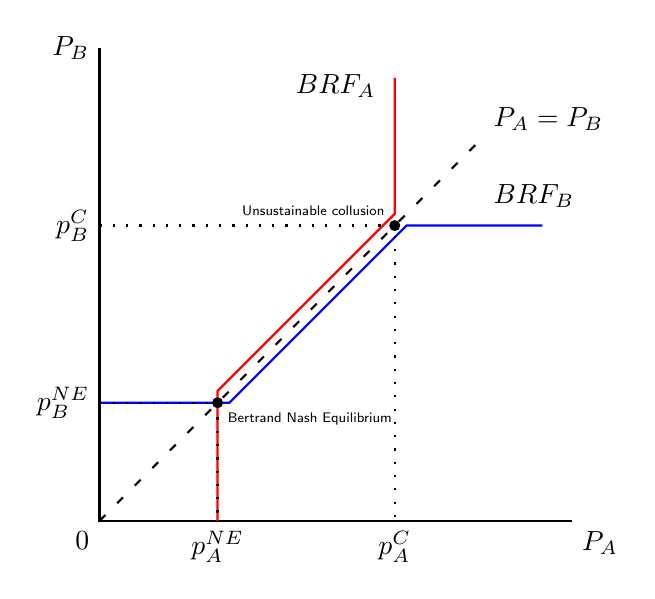
\begin{tikzpicture}[thick,font=\sffamily,scale=1.5]
	%axis
	\draw (0,4) node[left]{$P_{B}$} -- (0,0) node[below left] {$0$} -- (4,0) node[below right]{$P_{A}$}; %labels
	
	%BRFs
	\draw[red] (1,0) -- (1,1.1) -- (2.5,2.6)-- (2.5,3.75); %BRF A 
	\draw[blue] (0,1) -- (1.1,1) -- (2.6,2.5) -- (3.75,2.5); %BRFB

	 
	 %dotted lines
	 \draw [loosely dashed] plot[domain=0:3.25,smooth] (\x,\x); %y=x line
	 \draw[loosely dotted] (0,1) node[left]{$p^{NE}_B$} -| node[pos=0.25,below=3mm] {}
	  (1,0) node[below]{$p^{NE}_A$}; %Bertrand NE
	 \draw[loosely dotted] (0,2.5) node[left]{$p^{C}_B$} -| node[pos=0.25,below=3mm] {}
	  (2.5,0) node[below]{$p^{C}_A$}; %collusion
	  
	%labels
	\node[above] at (2,3.5) {$BRF_{A}$}; %BRF A label
	\node[right] at (3.25,2.75) {$BRF_{B}$}; %BRF B label
	\node[right] at (3.25,3.4) {$P_{A}=P_{B}$}; %y=x label
	
	%dots
	\node[style={fill=black,circle,inner sep=0pt,minimum size=4pt}] at (1,1) { };Bertrand NE
	\node[below right]at (1,1) {\tiny{Bertrand Nash Equilibrium}};
	\node[style={fill=black,circle,inner sep=0pt,minimum size=4pt}] at (2.5,2.5) { };SR equib
	\node[above left]at (2.5,2.5) {\tiny{Unsustainable collusion}}; %as the BRFs do not cross
	
\end{tikzpicture}
\end{document}